\section{Лекция 1 24.02.25. Численные методы решения нелинейных уравнений и систем}
\subsection{Постановка задачи}
Пусть $\mathbf{x} = \begin{pmatrix} 
x_1    \\ 
x_2    \\ 
\vdots \\ 
x_n    
\end{pmatrix} \in \mathbb{R}^n, F \in C(\mathbb{R}^n).
$
Дано уравнение:
\begin{equation}
	F(\mathbf{x}) = 0. 
\end{equation}
Требуется найти вектор $\mathbf{x}^* \in \mathbb{R}^n$ такой, что $F(\mathbf{x}^*) = 0$.
\subsection{Проблемы в вычислительном контексте}
\paragraph{Устойчивость.}
Пусть мы имеем уравнение
\[
	x^2 + px + q = 0.
\]
Известно, что если $p^2 = 4q$,
то уравнение имеет единственное решение.
Если в вычислительном эксперименте вместо $p$ и $q$ получить $p^*$ и $q^*$ соответственно, то могут появиться ложные решения или пропасть настоящие.
\paragraph{Построение $\varepsilon$-решения.}
\paragraph{Определение ($\varepsilon$-решение).} Вектор $\mathbf{x}^*$, удовлетворяющий неравенству
$
\|F(\mathbf{x}^*)\| < \varepsilon,
$
называется \textbf{$\varepsilon$-решением уравнения} (1).

Откуда брать $\varepsilon$? Универсальной процедуры нет. Нужно брать значение, соответствующее прогрешности, исходя из природы задачи.
\paragraph{Пример (подбор $\varepsilon$).} 
$\varepsilon = 1,6 \cdot 10^{-19}$ Кл. (уравнение электронного заряда).
\paragraph{Недостаточность $\varepsilon$-решения.}
\begin{center}
	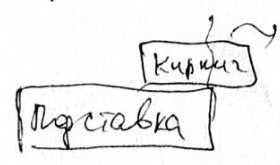
\includegraphics[width=5.2cm]{../figures/lection_1/figure_1.png}
\end{center}
Кирпич, стоящий на подставке --- система в состоянии неустойчивого равновесия. Нас интересует поиск момента фазового перехода (момента, когда кирпич упадёт), точно так же как для плавления, кристаллизации, таяния и других примеров систем. В теории динамических систем это называют точкой бифуркации. Если мы найдём $\varepsilon$-решение, оно не подойдёт, так как нужно, чтобы произошёл <<переход через ноль>>, иначе решение не будет представлять ценности. Может быть найдена не одна точка $x^*$, а интервал.
\paragraph{Определение (точка перехода через ноль в одномерном случае).} $x^*$ --- \textbf{точка перехода через ноль} для $f\in C(\mathbb{R})$, если $\forall \varepsilon > 0 \  f(x^*-\varepsilon)f(x^*+\varepsilon) < 0$.
\subsection{Переход через ноль в многомерном случае}
Пусть $M \subset \mathbb{R}^n$.
\paragraph{Определение (векторное поле).} $\varphi:M\rightarrow\mathbb{R}^n$ --- \textbf{векторное поле}.
\paragraph{Определение (особая точка).} $\mathbf{x}^*$ --- \textbf{особая точка}, если $\varphi(\mathbf{x}^*)=\mathbf{0}$.
\paragraph{Определение (изолированная особая точка).} Особая точка $\mathbf{x}^*$ --- \textbf{изолированная}, если $\exists \delta > 0 \  \forall \mathbf{x'}: (\vert\mathbf{x}^*-\mathbf{x'}\vert<\delta \implies \mathbf{x'}$ --- не особая).
\paragraph{Определение (устойчивая особая точка).} Особая точка называется \textbf{устойчивой}, если $\forall \delta > 0 \ \exists \tau > 0$: сдвиг поля на $\delta$ сдвинет особую точку не более, чем на $\tau$.
\\

Задача: найти устойчивые особые точки.
Введём характеристику, которая поможет найти переход через ноль.
Пусть $D \subset \mathbb{R}^n$ --- ограниченное. $\partial D$ --- граница этого множества. $\varphi$ --- невырожденное на $\partial D$ (т.е. нет особых точек).
Пусть $\mathbf{x}=(x_1,x_2,\hdots,x_n) \in \partial D$. Зададим параметризацию границы.
\[
	\left\{
	\begin{aligned}
		x_1 & = x_1(u_1, u_2, \dots, u_{n-1}) \\
		x_2 & = x_2(u_1, u_2, \dots, u_{n-1}) \\
		    & \hdots                          \\
		x_n & = x_n(u_1, u_2, \dots, u_{n-1}) 
	\end{aligned}
	\right.
\]
\paragraph{Пример (параметризация границы сферы).} $\left\{
\begin{aligned}
	x & = \rho \cos(\psi) \cos(\theta) \\
	y & = \rho \cos(\psi) \sin(\theta) \\
	z & = \rho \sin(\psi)              
\end{aligned}
\right.$
\\

Пусть $S_n$ --- площадь поверхности единичной сферы в $\mathbb{R}^n$.
\[
	\gamma(\varphi, \partial D) = \frac{1}{S_n} \int\limits_{\partial D} \frac{1}{\|\varphi(\mathbf{x})\|^n} \begin{vmatrix} \varphi_1(\mathbf{x}) & \frac{\partial \varphi_1(\mathbf{x}}{\partial u_1}  &\hdots & \frac{\partial \varphi_1(\mathbf{x}}{\partial u_{n-1}} \\ \varphi_2(\mathbf{x}) & \frac{\partial \varphi_2(\mathbf{x}}{\partial u_1}  &\hdots & \frac{\partial \varphi_2(\mathbf{x}}{\partial u_{n-1}} \\ \hdots & \hdots & \hdots & \hdots \\ \varphi_n(\mathbf{x}) & \frac{\partial \varphi_n(\mathbf{x}}{\partial u_1}  &\hdots & \frac{\partial \varphi_n(\mathbf{x}}{\partial u_{n-1}} \end{vmatrix} du_1du_2\hdots du_n.
\]
\paragraph{Определение (вращение векторного поля по границе).} Величина $\gamma(\varphi, \partial D)$ называется \textbf{вращением векторного поля $\varphi$ по границе $\partial D$}.
\paragraph{Упражнение.} Почему это называется вращением? Подсказка: рассмотрите двумерный случай, простое векторное поле $\varphi(\mathbf{x}) = \mathbf{x}$ и множество $D$ с границей, являющейся окружностью. Показать, что в двумерном случае это количество оборотов вектора поля при движении точки аргумента в положительном направлении по области границы.
\paragraph{Утверджение.} $\mathbf{x}^*$ --- изолированная особая точка, $S_1, S_2$ --- малые сферы вокруг $\mathbf{x}^*$. Тогда верно $\gamma(\mathbf{x}^*, \partial S_1) = \gamma(\mathbf{x}^*, \partial S_2) \implies ind(\mathbf{x}^*) := \gamma(\mathbf{x}^*, \partial S_i) \ \forall i$ --- \textbf{индекс особой точки}.
\paragraph{Теорема.} Изолированная особая точка устойчива $\iff$ $ind(\mathbf{x}) \neq 0$.
\paragraph{Упражнение.} Показать, что особая точка решения квадратного уравнения $x^2+px+q=0$ при $p^2=4q$ не обладает устойчивостью.
\subsection{Метод Чебышёва}
\paragraph{Постановка задачи.}
Решить $F(\mathbf{x}) = 0 \implies$ найти $\mathbf{x}^*: \|F(\mathbf{x}^*)\|<\varepsilon, ind(\mathbf{x}^*) \neq 0$.
Если интересуют все решения, то нужно найти множество $\varepsilon$-решений и границы интервалов ненулевого индекса.
Когда ищем так, о перечисленных проблемах 1.2.1 - 1.2.3 думать не нужно.
\paragraph{Условия метода.}
$F(x)=0; F \in C[a; b]; F(a)F(b) < 0 \implies \exists x^* \in [a; b]: F(x^*)=0$ (по т. Больцано-Коши).

\paragraph{Дополнительные ограничения.}
\begin{enumerate}
	\item $\forall x \in [a; b]\ \left| F'(x) \right| \ge \delta > 0 \implies \exists \varphi = F^{-1}$ и $\varphi$ имеет столько же непрерывных производных, сколько и $F$. (т. об обратном отображении)
	\item $F$ имеет $(m+1)$ непрерывных производных, $m = const$ (сильное требование!)
\end{enumerate}
\paragraph{Процедура метода.}
\[
	x^* \text{ --- решение } \implies F(x^*) = 0 \implies x^* = \varphi(0).
\]

Пусть $x_0$ --- произвольная фиксированная точка. $y_0 = F(x_0)$, $\hat{y}$ --- между $y$ и $y_0$.

По формуле Тейлора
\[
	\varphi(y) = \sum\limits_{k = 0}^m \frac{1}{k!} \frac{\partial^k \varphi(y_0)}{\partial y^k} (y-y_0)^k + \frac{1}{(m+1)!}\frac{\partial^{m+1}\varphi(\hat{y})}{\partial y^{m+1}}(y-y_0)^{m+1}.
\]

Пусть $y=0$. Тогда
\[
	x^* = \varphi(y_0) + \sum\limits_{k = 1}^m \frac{1}{k!} \frac{\partial^k \varphi(y_0)}{\partial y^k}(-y_0)^k + r_{m+1}(y_0).
\]

\[
	x^* = x_0 + \sum\limits_{k = 1}^m \frac{1}{k!} \frac{\partial^k \varphi(y_0)}{\partial y^k}(-y_0)^k + r_{m+1}(y_0).
\]

Пусть $x_1 = x^* - r_{m+1}(y_0)$.

Пусть $y_1 = F(x_1)$.

Применим снова формулу Тейлора в окрестности $y_1$.
\[
	x^* = x_1 + \sum\limits_{k=1}^m \frac{1}{k!}\frac{\partial^k\varphi(F(x_1))}{\partial y^k}((-F(x_1))^k) + r_{m+1}(y_1).
\]

Пусть $x_2 = x^* - r_{m+1}(y_1)$.

Пусть $y_2 = F(x_2)$.

Понятно, что $\vert x^* - x_{n}\vert \leq \vert r_{m+1}(y_1) \vert$.


Надежда (увы, это не всегда так):
\begin{enumerate}
	\item $x_n \in [a; b]$
	\item $x_n \underset{n \to \infty}{\longrightarrow} x^*$
\end{enumerate}

Как считать $\frac{\partial^k \varphi(F(x_i))}{\partial y^k}$?
\begin{enumerate}
	\item $y=F(x)$. $\varphi(F(x)) = x$. $\varphi'_y (F(x))F'(x) = 1 \implies \frac{\partial \varphi (F(x))}{\partial y} = \frac{1}{F'(x)}$, $F'(x)$ отдалена от нуля
	\item $\frac{d}{dx}[\varphi'_y (F(x))F'(x)] = 0$. $\varphi'_y (F(x))(F'(x))^2 + \varphi'_y (F(x))F''(x) = 0 \implies \frac {\partial^2 \varphi(F(x))}{\partial^2 y}$ можно выразить: $\varphi''_y (F(x)) = - \frac {\varphi'_y(F(x))F''(x)}{(F'(x))^2}$
\end{enumerate}


На сходимость сложно сформулировать какие-то внятные условия в общем виде.

\paragraph{Метод Ньютона.}
При $m=1$ мы имеем дело с ранее рассмотренным методом Ньютона. 
\[
	x_{n+1} = x_n - \frac{F(x_n)}{F'(x_n)}.
\]
Метод может не сходиться, но иногда работает.
\begin{center}
	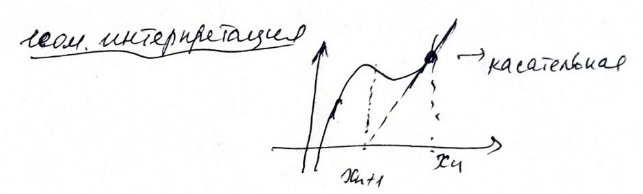
\includegraphics[width=8.2cm]{../figures/lection_1/figure_2.png}
\end{center}

\paragraph{Пример 1.}
\[
	x^2=a.
\]
\[
	F(x) = x^2 - a.
\]
\[
	F'(x) = 2x.
\]
\[
	x_{n+1} = x_n - \frac{x^2_n - a}{2x_n} = \frac{1}{2}(x_n+\frac{a}{x_n}).
\] --- метод Герона нахождения квадратных корней.

\paragraph{Пример 2.}
\[
	\sqrt[3]{x}e^{-x} = 0.
\]
Единственное решение $x^* = 0$. 
\[
	F(x) = x^{\frac{1}{3}} e^{-x}; F'(x) = \frac{1}{3}x^{-\frac{2}{3}}e^{-x} - x^{\frac{1}{3}}e^{-x}.
\] 
$\forall x_0$ метод Ньютона не сходится к решению.

Функции, на которых плохо работает метод Ньютона, обсуждаются в статье <<Pathological functions for Newton's method>> (1993).

\subsection{Метод простой итерации}
Приведём уравнение к виду $x = f(x)$.
\paragraph{Метод.} \begin{enumerate}
\item Выберем случайное $x_0$ --- начальное приближение
\item $x_{n+1} = f(x_n)$
\end{enumerate}
\paragraph{Дополнительные ограничения.} \begin{itemize}
\item Пусть $\delta$ --- фиксированное число. $\Omega\delta = \{x_0: \vert x - x_0 \vert < \delta \}$. Тогда $f$ должна быть определена в $\Omega \delta$
\item $\forall x', x'' \in \Omega\delta: \vert f(x'') - f(x') \vert < L\vert x'' - x' \vert, L < 1$ --- условие Липшица
\end{itemize}
Докажем существование и единственность решения.
Пусть $m = \vert f(x_0) - x_0 \vert$.
\[
	\vert x_1 - x_0\vert = m \implies (m < \delta \implies x_1 \in \Omega\delta).
\]
\[
	\vert x_2 - x_1\vert = \vert f(x_1) - f(x_0) \vert < L \vert x_1 - x_0 \vert < Lm.
\]
\[
	\vert x_2 - x_0\vert \leq \vert x_2 - x_1 \vert + \vert x_1 - x_0 \vert < Lm + m = (L + 1)m \implies (m(L+1) < \delta \implies x_2 \in \Omega\delta).
\]
Проведём нужное количество шагов до получения $x_n$.
\[
	\vert x_{n+1} - x_n \vert = L^n m.
\]
\[
	\vert x_{n+1} - x_0\vert = (1+L+\hdots+L^n)m = \frac{1}{1-L}m \implies (\frac{m}{1-L} < \delta \implies x_n \in \Omega \delta).
\]
\[
	\vert x_{n+k}-x_n\vert \leq \vert x_{n+k} - x_{n+k-1}\vert + \vert x_{n+k-1} - x_{n+k-2}\vert + \hdots + \vert x_{n+1} - x_n \vert < L^n m (1+L+\hdots+L^{k-1}) \leq
\]
\[
	\leq \frac{mL^n}{1-L} \underset{n \to \infty}{\longrightarrow} 0.
\]
Последовательность является сходящейся в себе (по Коши) $\implies \exists \underset{n \to \infty}{x_n} = x^*$.
$\forall n: x_n \in \Omega\delta \implies x^* \in \Omega\delta$.
\[
	f \in C(\mathbb{R}) \implies \underset{n\to\infty}{f(x_n)}=f(x^*)\implies\underset{n\to\infty}{f(x_{n+1})}=f(x^*)\implies f(x^*)=x^*.
\]
Существование решения доказано.
\[
	\vert x_{n+k} - x_n \vert < \frac{m}{1-L}L^n\implies \vert x_n - x^*\vert < \frac{m}{1-L}L^n = \frac{\vert f(x_0)-x_0\vert}{1-L}L^n.
\]
Пусть $x_1^*, x_2^*$ --- решения, $x_1^* \neq x_2^*$.
\[
	\vert x_1^* - x_2^* \vert = \vert f(x_1^*) - f(x_2^*)\vert < L\vert x_1^* - x_2^* \vert \implies L > 1 \ ?!
\]
Единственность решения доказана.
\paragraph{Теорема.} Пусть $f$ определена на $\Omega\delta$ и удовлетворяет условию Липшица с $L > 1$. Если $\frac{m}{1-L} < \delta$, то $\forall n: x_n \in \Omega \delta$ и метод простой итерации сходится к единственной неподвижной точке $x^*$, при этом верна оценка $\vert x_n - x^*\vert < \frac {m}{1-L}L^n$.
\subsection{Метод Ньютона решения систем}
Дана система.
\[
	\left\{
	\begin{aligned}
		f_1(x_1, x_2, \dots, x_{n}) & = 0    \\
		f_2(x_1, x_2, \dots, x_{n}) & = 0    \\
		                            & \hdots \\
		f_n(x_1, x_2, \dots, x_{n}) & = 0    
	\end{aligned}
	\right.
\]
Пусть $\mathbf{x}^0$ --- фиксированный вектор. $f_i(\mathbf{x}) = f_i(\mathbf{x}^0) + \sum\limits_{j = 1}^{n} \frac{\partial f_i(\mathbf{x^0})}{\partial x_j}(x_j-x^0_j) + r_i(\mathbf{x}, \mathbf{x^0})$ --- верно при условии непрерывности частных производных.
\[
	F'(\mathbf{x_0}) := \{\frac{\partial f_i(\mathbf{x^0})}{\partial x_j}\}_{i, j = 1}^n.
\]
\[
	F(\mathbf{x}) = F(\mathbf{x^0}) + F'(\mathbf{x^0})(\mathbf{x} - \mathbf{x^0}) + r(\mathbf{x}, \mathbf{x^0}).
\]
Пусть $x^*$ --- решение.
\[
	\mathbf{0} = F(\mathbf{x}^*) = F(\mathbf{x}^0) + F'(\mathbf{x}^0)(\mathbf{x}^* - \mathbf{x}^0) + r(\mathbf{x}^*, \mathbf{x}^0).
\]
Выкинем остаток.
\[
	F'(\mathbf{x}^0)(\mathbf{x}^*-\mathbf{x}^0) = -F(\mathbf{x}^0).
\]
\begin{equation}
	F'(\mathbf{x}^0)\mathbf{x}^* = F'(\mathbf{x}^0)\mathbf{x}^0 - F(\mathbf{x}^0).
\end{equation}
Левая часть равенства (2) --- матрица линейного оператора, а правая --- вектор. Таким образом, мы имеем СЛАУ с матрицей $F'(\mathbf{x}^0)$. Если данная система разрешима, будем называть её решением $\mathbf{x}^1$. Тогда $\mathbf{x}^2$ можно будет найти как решение следующей системы:
\[
	F'(\mathbf{x}^1)(\mathbf{x}-\mathbf{x}^1) = -F(\mathbf{x}^1).
\]
Нас интересуют следующие вопросы:
\begin{enumerate}
	\item Принадлежит ли $\mathbf{x}^k$ области определения $f$?
	\item Сходится ли $\mathbf{x}^k$ к $\mathbf{x}^*$?
	\item Единственность $\mathbf{x}^*$
\end{enumerate}
Эти условия, как и в методе простой итерации, можно указать. Мы, считая, что всё хорошо, просто оценим порядок сходимости, используя подчинённые нормы. $x \in \mathbb{R}^n, A \in M(m \times n)$.
\[
	\|x\| = \underset{i}{\max}\vert x_i \vert.
\]
\[
	\|A\|_\infty = \underset{i}{\max}\sum\limits_{j=1}^n\vert a_{ij} \vert.
\]
Построим оценку малости норм $\|r(\mathbf{x}^k, \mathbf{x}^*\|$.
\[
	\|r(\mathbf{x}+\Delta \mathbf{x}, \mathbf{x})\| = \|F(\mathbf{x} + \Delta \mathbf{x}) - F(\mathbf{x}) - F'(\mathbf{x}) \Delta \mathbf{x}\|.
\]
\[
	\varphi_i(\nu) := f_i(\mathbf{x} + \nu\Delta\mathbf{x}).
\]
\[
	\frac{d \varphi_i(\nu)}{d \nu} = \sum\limits_{j = 1}^n \frac{\partial f_i(\mathbf{x} + \nu\Delta\mathbf{x})}{\partial x_j}\Delta x_j \implies \int\limits_0^1 (\frac{\partial f_i(\mathbf{x} + \nu\Delta\mathbf{x})}{\partial x_j} \Delta x_j)d\nu = f_i(\mathbf{x} + \Delta\mathbf{x}) - f_i(\mathbf{x}) \implies
\]
\[
	\implies \vert f_i(\mathbf{x}+\Delta\mathbf{x}) - f_i(\mathbf{x}) - \sum\limits_{j = 1}^n \frac{\partial f_i(\mathbf{x})}{\partial x_j}\Delta x_j\vert =  \vert\int\limits_0^1(\frac{\partial f_i(\mathbf{x} + \nu\Delta\mathbf{x})}{\partial x_j}\Delta x_j)d\nu - \int\limits_0^1(\frac{\partial f_i(\mathbf{x})}{\partial x_j})d\nu\vert =
\]
\[
	= \vert \int\limits_0^1 ((\frac{\partial f_i(\mathbf{x} + \nu\Delta\mathbf{x})}{x_j} - \frac{\partial f_i(\mathbf{x})}{\partial x_j})\Delta x_j)d\nu\vert \leq \int\limits_0^1\vert\sum\limits_{j=1}^n(\frac{\partial f_i(\mathbf{x} + \nu\Delta\mathbf{x})}{\partial x_j} - \frac{\partial f_i(\mathbf{x})}{\partial x_j})\Delta x_j\vert d\nu \leq
\]
\[
	\leq \int\limits_0^1 \sum\limits_{j = 1}^n \vert \frac{\partial f_i(\mathbf{x} + \nu\Delta\mathbf{x})}{\partial x_j} - \frac{\partial f_i(\mathbf{x})}{\partial x_j}\vert \vert \Delta x_j \vert d\nu \leq \|\Delta \mathbf{x}\| \int\limits_0^1 \sum\limits_{j = 1}^n \vert \frac{\partial f_i(\mathbf{x} + \nu\Delta\mathbf{x})}{\partial x_j} - \frac{\partial f_i(\mathbf{x})}{\partial x_j} \vert d\nu =
\]
\[
	= \| F'(\mathbf{x} + \nu\Delta\mathbf{x}) - F'(\mathbf{x})\|.
\]
Пусть $F'$ удовлетворяет условию Липшица, то есть $\forall x', x'': \|F'(\mathbf{x}'')\ - F'(\mathbf{x}')| \leq L\|\mathbf{x}'' - \mathbf{x}'\|$. Тогда
\[
	\|F(\mathbf{x} + \Delta\mathbf{x}) - F(\mathbf{x}) - F'(\mathbf{x})\Delta\mathbf{x}\| \leq \|\Delta\mathbf{x}\|\int\limits_0^1\|F'(\mathbf{x} + \Delta\mathbf{x}) - F'(\mathbf{x})\|d\nu \leq \|\Delta\mathbf{x}\|\int\limits_0^1L\nu\|\Delta\mathbf{x}\|d\nu \leq \frac{1}{2}L\|\Delta\mathbf{x}\|^2.
\]
Пусть $\mathbf{x}^k \underset{k \to \infty}{\longrightarrow} \mathbf{x}^*$ и $\mathbf{x}^{k + 1}$ --- решение. Известно равенство $F'(\mathbf{x}^k)(\mathbf{x}-\mathbf{x}^k) = -F(\mathbf{x}^k)$.
\begin{itemize}
	\item $F'(\mathbf{x})$ удовлетворяет условию Липшица
	\item $\|(F'(\mathbf{x}))^{-1}\| \leq \eta > 0$
\end{itemize}
Пусть $y = -F(\mathbf{x}^k) - F'(\mathbf{x}^k)(\mathbf{x}^* - \mathbf{x}^k)$. 
\[
	y = -F(\mathbf{x}^k) - F'(\mathbf{x}^k)(\mathbf{x}^{k+1} - \mathbf{x}^k + \mathbf{x}^* - \mathbf{x}^{k + 1}) = -F'(\mathbf{x}^k)(\mathbf{x}^*-\mathbf{x}^{k+1}).
\]
Из обратимости оператора следует, что:
\[
	\mathbf{x}^k - \mathbf{x}^{k + 1} = -[F'(\mathbf{x}^k)]^{-1}y \implies \|\mathbf{x}^* - \mathbf{x}^{k + 1}\| \leq \eta\|y\| = \eta\|y + F(\mathbf{x}^*)\| =
\]
\[
	= \eta \|F(\mathbf{x}^* - F(\mathbf{x}^k) - F'(\mathbf{x}^k)(\mathbf{x}^*) - \mathbf{x}^k)\| \leq \eta \cdot L \|\mathbf{x}^* - \mathbf{x}^k\|^2 \implies
\]
\[
	\implies \| \mathbf{x}^* - \mathbf{x}^{k + 1}\| \leq \frac{1}{2}L\eta\|\mathbf{x}^* - \mathbf{x}^k\|^2.
\]
В таком случае говорят, что порядок сходимости метода равен двум.
На практике применяются Jacobian-free methods, отказ от $F'(\mathbf{x}), [F'(\mathbf{x})]^{-1}$. Эти методы обсуждаются в статье <<Jacobian-free Newton–Krylov methods: a survey of approaches and applications>> (2004).
